\documentclass[10pt]{beamer}

\usetheme[progressbar=frametitle, numbering=fraction,]{metropolis}

\usepackage{booktabs}
\usepackage{pgfplots}
\usepgfplotslibrary{dateplot}
\usepackage{texshade}      
\usepackage{amsmath}
\usepackage{amssymb}
\usepackage{xspace}
\usepackage{xcolor}
\usepackage{appendixnumberbeamer}
\usepackage{multirow}

\usepackage{tikz}
\usetikzlibrary{shapes.geometric, arrows}
\tikzstyle{startstop} = [rectangle, rounded corners, minimum width=3cm, minimum height=1cm,text centered, draw=black, fill=red!30]
\tikzstyle{io} = [trapezium, trapezium left angle=70, trapezium right angle=110, minimum width=3cm, minimum height=1cm, text centered, draw=black, fill=blue!30]
\tikzstyle{process} = [rectangle, minimum width=3cm, minimum height=1cm, text centered, draw=black, fill=orange!30]
\tikzstyle{decision} = [diamond, minimum width=3cm, minimum height=1cm, text centered, draw=black, fill=green!30]

\tikzstyle{arrow} = [thick,->,>=stealth]


\newcommand{\themename}{\textbf{\textsc{metropolis}}\xspace}

\setbeamercovered{invisible}
\setbeamertemplate{caption}{\raggedright\insertcaption\par}

\title{Introduction to Scientific Research}
%\subtitle{What we see, is not what it is}
\date{\today}
\author{Saket Choudhary}
\institute{BISC 104\\Session 1}
%\titlegraphic{\hfill\includegraphics[height=1.5cm]{logo}}

\begin{document}

\maketitle

\begin{frame}[fragile]
  \Large\begin{center}Scientific research probes deepest mysteries\\
  of universe
  \end{center}
  \
\end{frame}

\begin{frame}[fragile]{The Process}
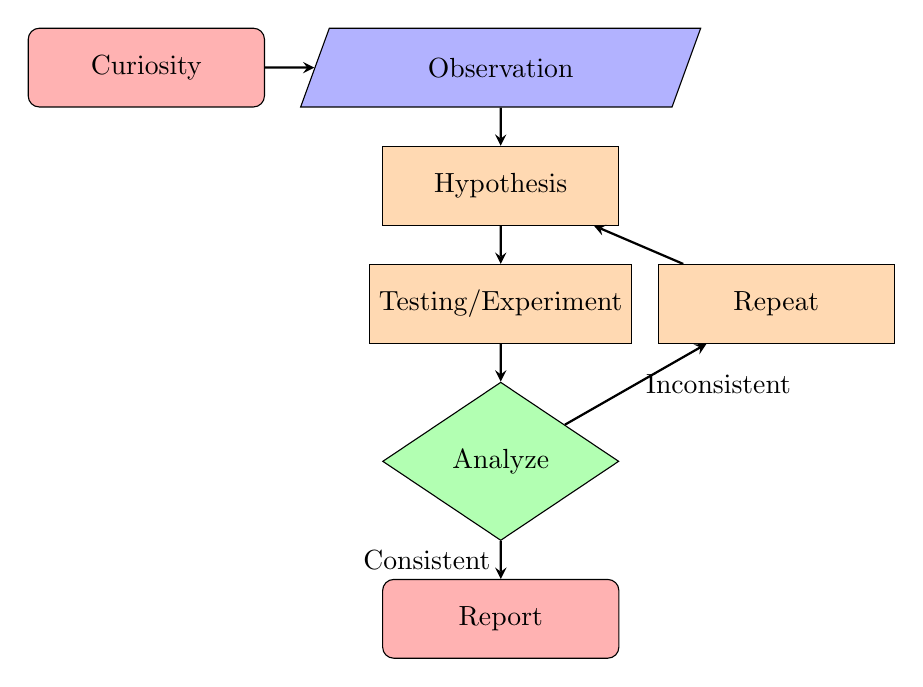
\begin{tikzpicture}[node distance=1.5cm, scale=0.1]
\node (start) [startstop] {Curiosity};
\node (in1) [io, right of=start, xshift=3cm] {Observation};
\node (pro1) [process, below of=in1] {Hypothesis};
\node (pro2) [process, below of=pro1] {Testing/Experiment};
\node (dec1) [decision, below of=pro2, yshift=-0.5cm] {Analyze};
\node (end) [startstop, below of=dec1, yshift=-0.5cm] {Report};
\node (rep1) [process, right of=pro2, xshift=2cm] {Repeat};


\draw[arrow] (start) --  (in1);
\draw[arrow] (in1) --  (pro1);
\draw[arrow] (pro1) --  (pro2);
\draw[arrow] (pro2) --  (dec1);
\draw [arrow] (dec1) -- node[anchor=east] {Consistent} (end);
\draw [arrow] (dec1) -- node[anchor=west] {Inconsistent} (rep1);
\draw [arrow] (rep1) -- (pro1);

\end{tikzpicture}
\end{frame}

\begin{frame}[fragile]{Elements of an experiment}
\begin{itemize}[<+- | alert@+>]
\item \textbf{Independent variable}: Intentionally manipulated by experimenter
\item \textbf{Dependent variable}: Changes due to change in independent variable [Measured/Observed]
\item \textbf{Control variable}: Could possible affect dependent variable, so should be kept constant
\end{itemize}

\end{frame}


\begin{frame}[fragile]{Example: Baking bread}
\begin{itemize}[<+- | alert@+>]
\item \textbf{Hypothesis:} If amount of sugar increases, bread rises higher
\item \textbf{Independent Variable}: Amount of sugar
\item \textbf{Dependent Variable}: Size of loaf
\item \textbf{Control Variables}: Water, salt, temperature, brand of ingredients ... Should remain constant

\end{itemize}
\begin{center}
\uncover<5->{
\begin{table}

\begin{tabular}{l|l|l}
Amount of Sugar & Size of bread\\
\hline
10g & 600$cm^2$ \\
20g & 700$cm^2$ \\
25g & 710$cm^2$ \\
30g & 715$cm^2$ \\
\end{tabular}
\caption{Analysis Table}
\end{table}
Sample Size?\\ 
Variability?
\end{center}}

\end{frame}

\begin{frame}[fragile]{Example: Fertilizer and yield}
\begin{itemize}[<+- | alert@+>]
\item \textbf{Hypothesis:} Fertilizer X gives a better yield over fertilizer $Y$
\item \textbf{Independent Variable:} Amount of fertilizers X,Y
\item \textbf{Dependent Variable:} Yield [kg/tonnes..]
\item \textbf{Control Variables:} Watering frequency, temperature, weather conditions ....
\end{itemize}

\end{frame}

\begin{frame}[fragile]{Today's Plan}
\begin{itemize}[<+- | alert@+>]
\item Split into 4 groups
\item Come up with proposals \textbf{that can be tested} and involves watching people at USC
\item All groups vote to select the best proposal
\item Form groups of 2, decide a day/time to collect data
\item Disperse!
\item Carry out your experiments, analyze your results.
\end{itemize}
\uncover<6->{
We will go over analysis part in next session.
Please email your analysis report by next Tuesday 5PM.}
\end{frame}


%\begin{frame}[fragile]{Possible Analysis Table}
%\begin{table}
%\begin{tabular}{c|c|c}
%Time-Day & \# Males & \# Females\\
%\hline
%1215-1245--Th & .. & ..\\
%1310-1340--W  & .. & ..\\
%\hline
%Total & .. & ..
%\end{tabular}
%\end{table}
%\end{frame}

\begin{frame}[fragile]{Office Hours}
\Large \begin{center}Tuesday: 9-10AM\\
Wednesday: 9-10AM\\
ZSH 372\\
\vspace*{2cm}
Saket Choudhary\\ 
skchoudh@usc.edu\\
\end{center}

\textbf{Please don't forget to mail your analysis/report by 5PM, Tuesday(09/06).}

\end{frame}

\end{document}
